\documentclass[a4paper]{article}
\usepackage[a4paper,hmargin={3cm,2.5cm},vmargin={2.5cm,2.5cm}]{geometry}

\usepackage{tikz}
\usetikzlibrary{calc}

\usepackage{fancyhdr}
\pagestyle{fancy}
\lhead{}
\rhead{Computer Architecture \& Organization Laboratory}
\lfoot{Department of Computer Science \& Technology}

\usepackage{enumitem}


\usepackage{hyperref}

\usepackage{caption}
\usepackage{subcaption}

\usepackage{amsmath}

\usepackage{cleveref}




\begin{document}
\begin{titlepage}
    \begin{tikzpicture}[overlay,remember picture]
        \draw[line width=4pt]
        ($ (current page.north west) + (1cm,-1cm) $)
        rectangle
        ($ (current page.south east) + (-1cm,1cm) $);
        \draw[line width=1.5pt]
        ($ (current page.north west) + (1.2cm,-1.2cm) $)
        rectangle
        ($ (current page.south east) + (-1.2cm,1.2cm) $);
    \end{tikzpicture}
    
    \begin{center}

        \textup{\large  \textbf{INDIAN INSTITUTE OF ENGINEERING}\\\textbf{SCIENCE AND TECHNOLOGY, SHIBPUR}}\\ 
        Howrah, West Bengal, India - 711103\\[1cm]
        
        \textbf{\large DEPARTMENT OF COMPUTER SCIENCE}\\
        \textbf{\large AND TECHNOLOGY}\\[1cm]
        
        %---------------------------------Figure------------------------------
        \begin{center}
            \begin{figure}[h]   %h means here other options t , b, p, etc.
                \centering
                
\includegraphics[width=0.3\linewidth]{Pictures/IIESTS Logo.png}
            \end{figure}
        \end{center}
        
        %----------------------------
        
        \textup{\large Computer Architecture \& Organization Laboratory\\[0.4cm][CS2272]}\\[1cm]
        
        \begin{LARGE}
            {\textbf {LAB REPORT}}
        \end{LARGE}\\[1cm]
        
        \textit{SUBMITTED BY}\\[0.3cm]
        \begin{large}
            \textbf{Abhiroop Mukherjee (510510109)}\\[1cm]
        \end{large}
        
        \textit{UNDER THE GUIDANCE OF}\\[0.3cm]
        \begin{large}
            \textbf{PROF. BIPLAB K. SIKDAR}\\[0.3cm]
            \textbf{PROF. JAYA SIL}\\[1cm]
        \end{large}
        
        \textbf{(4th Semester, Academic Year: 2020-2021)}
    \end{center}
\end{titlepage}

%----------------------ACKNOWLEDGEMENT---------------------------
\pagebreak

\pagenumbering{roman}
\setcounter{page}{1}
\setcounter{tocdepth}{1} % + subsections
\tableofcontents
\newpage

\pagenumbering{arabic}
\setcounter{page}{1}



\section{Organization of $m\times d$ memory with Flip Flops}
\subsection{Objective}
To design memory module with the features of Read/Write, using RS Flip Flop, considering
\begin{enumerate}[label=(\alph*)]
    \item $m=1, d=1$
    \item $m=2, d=1$
    \item $m=2, d=2$, using the design resulted out of (b)
\end{enumerate}

\subsection{Theoretical Basis}
A $2^m\times d$ Memory Module can be drawn as follows
\begin{figure}[h!]
    \centering
    \includegraphics[width=0.4\linewidth]{Pictures/Experiment 1/Memory.jpg}
    \caption{A $m\times d$ Memory Module}
    \label{fig:MemModmd}
\end{figure}

Here CS is Chip Select  and $RD/\overline{WR}$ is Read or Write input.

Given an $2^m\times d$ Memory Module, we can make $2^{m+1}\times d$  and $2^m\times 2d$ Memory Modules as follows

\begin{figure}[h!]
    \centering
    \begin{subfigure}[b]{0.4\linewidth}
        \includegraphics[width=\linewidth]{Pictures/Experiment 1/2^(m+1)xd.jpg}
        \caption{A $2^{m+1}\times d$ Memory Module}
    \end{subfigure}
    \begin{subfigure}[b]{0.4\linewidth}
        \includegraphics[width=\linewidth]{Pictures/Experiment 1/2^m x 2d.jpg}
        \caption{A $2^m\times 2d$ Memory Module}
    \end{subfigure}
    \caption{Expansion of Memory Modules}
    \label{fig:ExpMemMod}
\end{figure}
\pagebreak

\subsection{Task}
To Realize Circuit of:
\begin{enumerate}[label=(\alph*)]
    \item 1 bit 1 word memory
    \item 1 bit 2 word memory
    \item 2 bit 2 word memory
\end{enumerate}

\subsection{Major Components/Modules Used}
\begin{enumerate}
    \item RS Flip Flop
    \item Tri-state logic
    \item Triple-input NAND Gate
    \item Inverter
\end{enumerate}

\subsection{Design}
Following the above Ideas, we construct required memory modules as follows

\begin{figure}[h!]
    \centering
    \begin{subfigure}[b]{0.45\linewidth}
        \centering
        \includegraphics[width=\linewidth]{Pictures/Experiment 1/1b1w.jpg}
        \caption{1 bit 1 word memory}
    \end{subfigure}
    \begin{subfigure}[b]{0.45\linewidth}
        \centering
        \includegraphics[width=\linewidth]{Pictures/Experiment 1/1b2w.jpg}
        \caption{1 bit 2 word memory}
    \end{subfigure}
    \begin{subfigure}[b]{\linewidth}
        \centering
        \includegraphics[width=0.85\linewidth]{Pictures/Experiment 1/2b2w.jpg}
        \caption{2 bit 2 word memory}
    \end{subfigure}
    \caption{Design Of Memory}
    \label{Fig:MemDes}
\end{figure}
\pagebreak

\subsection{Implementation}
\begin{figure}[h!]
    \centering
    \begin{subfigure}[b]{0.4\linewidth}
        \centering
        \frame{\includegraphics[width=\linewidth]{Pictures/Experiment 1/imp1b1w.jpg}}
        \caption{1 bit 1 word memory}
    \end{subfigure}
    \begin{subfigure}[b]{0.4\linewidth}
        \centering
        \frame{\includegraphics[width=\linewidth]{Pictures/Experiment 1/imp1b2w.jpg}}
        \caption{1 bit 2 word memory}
    \end{subfigure}
    \begin{subfigure}[b]{\linewidth}
        \centering
        \frame{\includegraphics[width=\linewidth]{Pictures/Experiment 1/imp2b2w.jpg}}
        \caption{2 bit 2 word memory}
    \end{subfigure}
    \caption{Implementation Of Memory}
    \label{Fig:MemImp}
\end{figure}
\pagebreak

\subsection{Verification/Simulation}

\begin{table}[h!]
    \begin{center}
        \begin{tabular}{|c|c|c|c|c|c|}
            \hline
            \textbf{Sr. No} & \textbf{Select} & \textbf{R/$\overline{W}$} & \textbf{Data In} & \textbf{Data Out} & \textbf{Activity} \\
            \hline
            1               & 1               & 0                         & 1                & -                 & Write 1 in Loc-1  \\
            2               & 1               & 1                         & -                & 1                 & Read 1 from Loc-1 \\
            3               & 0               & x                         & -                & -                 & No operation      \\
            4               & 1               & 0                         & 0                & -                 & Write 0 in Loc-1  \\
            5               & 1               & 1                         & 1                & 0                 & Read 0 from Loc-1 \\
            \hline
        \end{tabular}
        \label{tab:1b1w}
        \caption{1 bit 1 word memory}
    \end{center}
\end{table}


\begin{table}[h!]
    \begin{center}
        \begin{tabular}{|c|c|c|c|c|c|}
            \hline
            \textbf{Sr. No} & \textbf{Select} & \textbf{R/$\overline{W}$} & \textbf{Data In} & \textbf{Data Out} & \textbf{Activity} \\
            \hline
            1               & 1               & 0                         & 1 ($d_1$)        & -                 & Write 1 in Loc-1  \\
            2               & 0               & 0                         & 1 ($d_2$)        & -                 & Write 1 in Loc-0  \\
            3               & 1               & 1                         & -                & 1  ($d_1$)        & Read 1 from Loc-1 \\
            4               & 0               & 1                         & -                & 1  ($d_2$)        & Read 1 from Loc-0 \\
            5               & 1               & 0                         & 0                & -                 & Write 0 in Loc-1  \\
            6               & 0               & 0                         & 1                & -                 & Write 1 in Loc-0  \\
            7               & 1               & 1                         & -                & 0                 & Read 0 from Loc-1 \\
            8               & 0               & 1                         & -                & 1                 & Read 1 from Loc-0 \\
            9               & 1               & 0                         & 1                & -                 & Write 1 in Loc-1  \\
            10              & 0               & 0                         & 0                & -                 & Write 0 in Loc-0  \\
            11              & 1               & 1                         & -                & 1                 & Read 1 from Loc-1 \\
            12              & 0               & 1                         & -                & 0                 & Read 0 from Loc-0 \\
            \hline
        \end{tabular}
        \label{tab:1b2w}
        \caption{1 bit 2 word memory}
    \end{center}
\end{table}

\begin{table}[h!]
    \begin{center}
        \begin{tabular}{|c|c|c|c|c|c|c|c|}
            \hline
            \textbf{Sr. No} & \textbf{Select} & \textbf{R/$\overline{W}$} & \textbf{$D1_{in}$} & \textbf{$D0_{in}$} & \textbf{$D1_{out}$} & \textbf{$D0_{out}$} & \textbf{Verify}    \\
            \hline
            1               & 1               & 0                         & 1                  & 0                  & -                   & -                   & Write 10 in Loc-1  \\
            2               & 0               & 0                         & 0                  & 1                  & -                   & -                   & Write 01 in Loc-0  \\
            3               & 1               & 1                         & -                  & -                  & 1                   & 0                   & Read 10 from Loc-1 \\
            4               & 0               & 1                         & -                  & -                  & 0                   & 1                   & Read 01 from Loc-0 \\
            5               & 1               & 0                         & 0                  & 0                  & -                   & -                   & Write 00 in Loc-1  \\
            6               & 0               & 0                         & 1                  & 1                  & -                   & -                   & Write 11 in Loc-0  \\
            7               & 1               & 1                         & -                  & -                  & 0                   & 0                   & Read 00 from Loc-1 \\
            8               & 0               & 1                         & -                  & -                  & 1                   & 1                   & Read 11 from Loc-0 \\
            \hline
        \end{tabular}
        \label{tab:2b2w}
        \caption{2 bit 2 word memory}
    \end{center}
\end{table}

\subsection{Conclusion}
We can design $2^{m_1} \ast d_1$ Memory Module where $m_1 >= m$ and $d_1 >= d$
\pagebreak


\section{Design of Carry-Look-Ahead Adder}

\subsection{Objective}
To Design
\begin{enumerate}
    \item 4-bit carry lookahead adder (CLA) using half adders/full adders.
    \item A 16-bit CLA using 4-bit CLAs.
\end{enumerate}

\subsection{Theoretical Basis and Design}
Basic Unit of Carry Look-Ahead Adder is as follows:
\begin{figure}[h!]
    \centering
    \includegraphics[width=0.2\linewidth]{Pictures/Experiment 2/CLA.jpg}
    \caption{Basic Unit of CLA}
    \label{fig:CLA}
\end{figure}

where,

\begin{align}
    p_i & = x_i \oplus y_i \nonumber \\\
    g_i & = x_{i}y_i       \nonumber
\end{align}

Using this building blocks, we can construct an n-bit CLA as follows

\begin{figure}[h!]
    \centering
    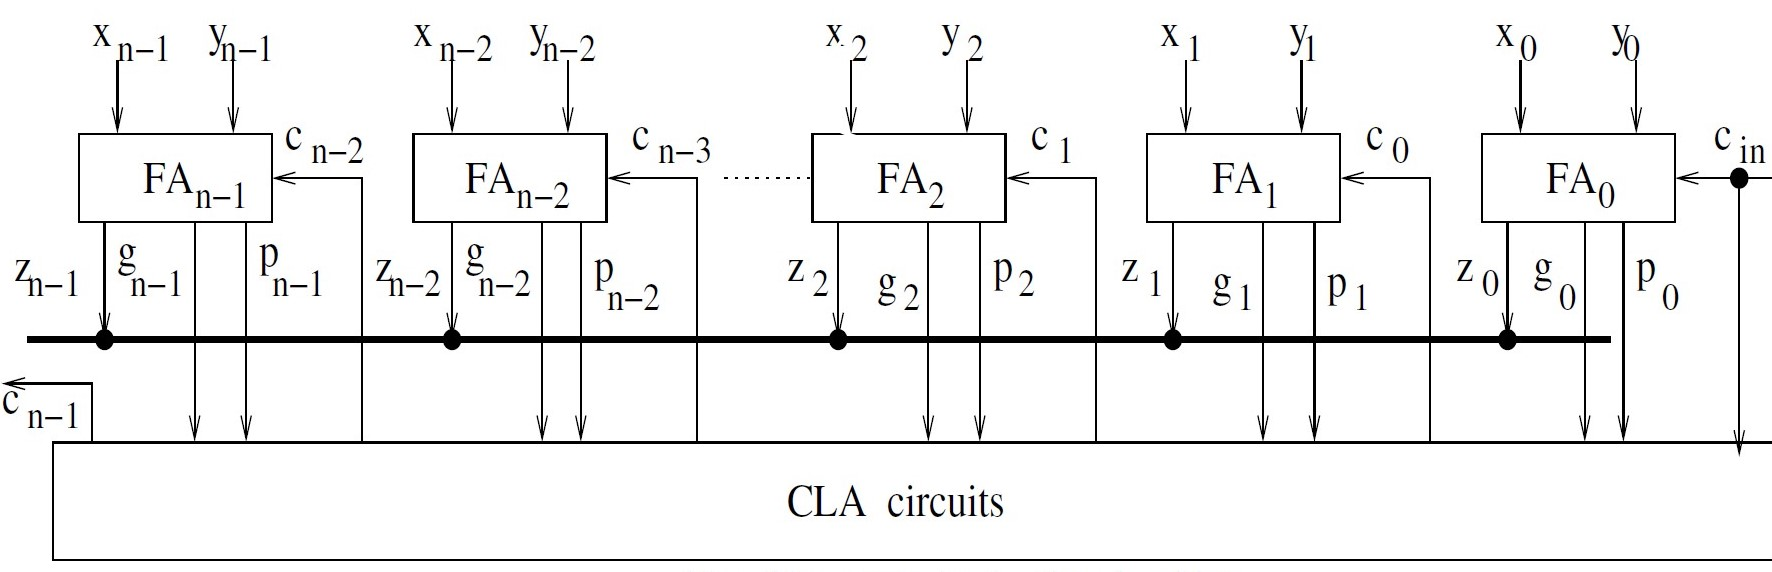
\includegraphics[width=\linewidth]{Pictures/Experiment 2/nbitCLA.jpg}
    \caption{n-bit CLA}
    \label{fig:nbitCLA}
\end{figure}
\pagebreak

Using these we can form this for 4-bit CLA

\begin{align}
    c_0 & = g_0 + p_0c_{in} \nonumber                                                              \\
    c_1 & = g_1 + p_1c_0 = g_1 + p_1g_0 + p_1p_0c_{in} \nonumber                                   \\
    c_2 & = g_2 + p_2c_1 = g_2 + p_2g_1 + p_2p_1g_0 + p_2p_1p_0c_{in} \nonumber                    \\
    c_3 & = g_3 + p_3c_2 = g_3 + p_3g_2 + p_3p_2g_1 + p_3p_2p_1g_0 + p_3p_2p_1p_0c_{in} \nonumber 
\end{align}

Now from 4-bit CLA, we can construct 16-bit CLA as follows:

\begin{figure}[h!]
    \centering
    \includegraphics[width=0.8\linewidth]{Pictures/Experiment 2/16bitCLA.jpg}
    \caption{16-bit CLA}
    \label{fig:16bitCLA}
\end{figure}


\subsection{Task}
\begin{enumerate}
    \item Construct 4 modules as in Figure \ref{fig:CLA} (can use half adder).
    \item Simplify the expressions for $c_0$, $c_1$, $c_2$ and $c_3$ assuming $c_{in}$ = 0.
    \item Design CLA circuits i.e, realize $c_0$, $c_1$, $c_2$ and $c_3$.
    \item Design the CLA as in Figure \ref{fig:nbitCLA} and verify a part of its truth table.
    \item Report on the design of a 16-bit CLA as in Figure \ref{fig:16bitCLA}.
\end{enumerate}

\subsection{Major Components/Modules Used}
\begin{enumerate}
    \item AND Gate
    \item OR Gate
    \item Half Adder
    \item Full Adder
\end{enumerate}
\pagebreak
\subsection{Implementation}
\begin{figure}[h!]
    \centering
    \begin{subfigure}[b]{\linewidth}
        \centering
        \frame{\includegraphics[width=0.4\linewidth]{Pictures/Experiment 2/ImpCLABlock.jpg}}
        \caption{Block of CLA Adder}
    \end{subfigure}
    \begin{subfigure}[b]{\linewidth}
        \centering
        \frame{\includegraphics[width=0.6\linewidth]{Pictures/Experiment 2/Imp4bitCLA.jpg}}
        \caption{4 bit CLA}
        \label{subFig:4bCLA}
    \end{subfigure}
    \begin{subfigure}[b]{\linewidth}
        \centering
        \frame{\includegraphics[width=\linewidth]{Pictures/Experiment 2/Imp16bitCLA.png}}
        \caption{16 bit CLA}
        \label{subFig:16bCLA}
    \end{subfigure}
    \caption{Carry Look Ahead Adder}
    \label{Fig:ImpCLA}
\end{figure}

\subsection{Verification}
\begin{itemize}
    \item We are successfully able to add two 4-bit numbers using circuit in Figure \ref{subFig:4bCLA}.
    \item We are successfully able to add two 16-bit numbers using circuit in Figure \ref{subFig:16bCLA}
\end{itemize}

\subsection{Conclusion}
We are able to add two 4-bit number in constant delay time and are able to add two 16-bit numbers in some delay, which is not proportional to number of bits.
\pagebreak

\section{Implementation of data movement instructions}

\subsection{Objective}
To realize data movement instructions in a CPU having four 2-bit registers.

\subsection{Theoretical Basis}

\hspace{0.5cm}Data movement instructions move data from one place, called the source operand, to another place, called the destination operand.

Data is transferred directly from a source register in a register file connected to a data bus from a destination register in the register file, through a data bus bypass mechanism.

The figure shown below shows how to implement such data movement instructions when the source register and the destination register belong to the same set of registers.

\begin{figure}[h!]
    \centering
    \includegraphics[width=0.8\linewidth]{Pictures/Experiment 3/regDataTran.jpg}
    \caption{Data Transfer between same set of Registers}
    \label{fig:regDataTran}
\end{figure}

\subsection{Task}

Given four 2-bit registers $R_0$, $R_1$, $R_2$, and $R_3$. We need to realize the implementation of data movement instruction like

\emph{MOV $\langle$dest reg addr$\rangle$ $\langle$source reg addr$\rangle$}

\noindent Here we set source and destination address manually

\subsection{Major Components/Modules Used}
\begin{enumerate}
    \item Four 4-bit Registers, but only using 2 MSB to essentially simulate 2-bit Register
    \item Two 4 to 1 Multiplexer
    \item One 2 of 4 Decoder
\end{enumerate}
\pagebreak

\subsection{Design}

\begin{figure}[h!]
    \centering
    \includegraphics[width=0.8\linewidth]{Pictures/Experiment 3/desDataTran.jpg}
    \caption{Design Idea to implement Data Transfer between four Registers}
    \label{fig:regDataTran}
\end{figure}

\subsection{Implementation}
\begin{figure}[h!]
    \centering
    \frame{\includegraphics[width=0.8\linewidth]{Pictures/Experiment 3/impDataTran.jpg}}
    \caption{Implementation of Data Transfer between four Registers}
    \label{fig:regDataTran}
\end{figure}

\subsection{Verification}
The circuit developed for the implementation of Data Transfer between Registers works as expected.\\
i.e. it moves 2-bit data from one register from the source register to destination register.

\subsection{Conclusion}
A circuit for the implementation of data movement between registers has been successfully designed and verified using simulation. Hence the assigned task is complete.
\pagebreak

\section{Swapping contents of registers using Microprogram}
\subsection{Objective}
To become familiar with
\begin{enumerate}[label=(\alph*)]
    \item Register level data transfer through common bus
    \item Microprogrammed realization of the register level data transfer
\end{enumerate}

\subsection{Theoretical Basis}

The $\mu$-programming is a method of designing a control unit in which control signal selection and sequencing information is stored in a ROM/RAM.
The control signals to be activated at time $t$ are specified by a $\mu$-instruction.
A sequence of $\mu$-instructions related to a task is the $\mu$-program. In the present design, the $\mu$-program is stored in memory/RAM.

\subsection{Task and Design}
\begin{enumerate}
    \item Setting registers and control switches (manually) to realize swapping of data:
    \begin{enumerate}
        \item Realize registers A, B and T with D latches/registers as in Figure \ref{subFig:d-swapAB}.
        \item Set the switches (control signals) C1, C2, and C3 to realize data swap.
        \item Identify additional control signals required to realize swapping through common bus.
    \end{enumerate}
    \item Automated swapping of data:
    \begin{enumerate}
        \item Realize bi-directional bus (Figure \ref{subFig:c-bus}).
        \item Identify the control signals required to realize the following sequence of $\mu$-instructions
        \begin{enumerate}
            \item Copy T$\leftarrow$A
            \item No operation
            \item Copy A$\leftarrow$B
            \item No operation
            \item Copy B$\leftarrow$T
        \end{enumerate}
    \end{enumerate}
    \item Setting up control memory:
    \begin{enumerate}
        \item Write $\mu$-instructions in memory. Generate memory address using counter. Supply clock to generate next addresses (Figure \ref{subFig:c-mem}).
        \item Rin $\mu$-program.
    \end{enumerate}
\end{enumerate}

\begin{figure}[h!]
    \centering
    \begin{subfigure}[b]{0.3\linewidth}
        \centering
        \includegraphics[width=\linewidth]{Pictures/Experiment 4/data-swap.jpg}
        \caption{Data Swap}
        \label{subFig:d-swapAB}
    \end{subfigure}
    \begin{subfigure}[b]{0.3\linewidth}
        \centering
        \includegraphics[width=\linewidth]{Pictures/Experiment 4/c-bus.jpg}
        \caption{Common Bus}
        \label{subFig:c-bus}
    \end{subfigure}
    \begin{subfigure}[b]{0.3\linewidth}
        \centering
        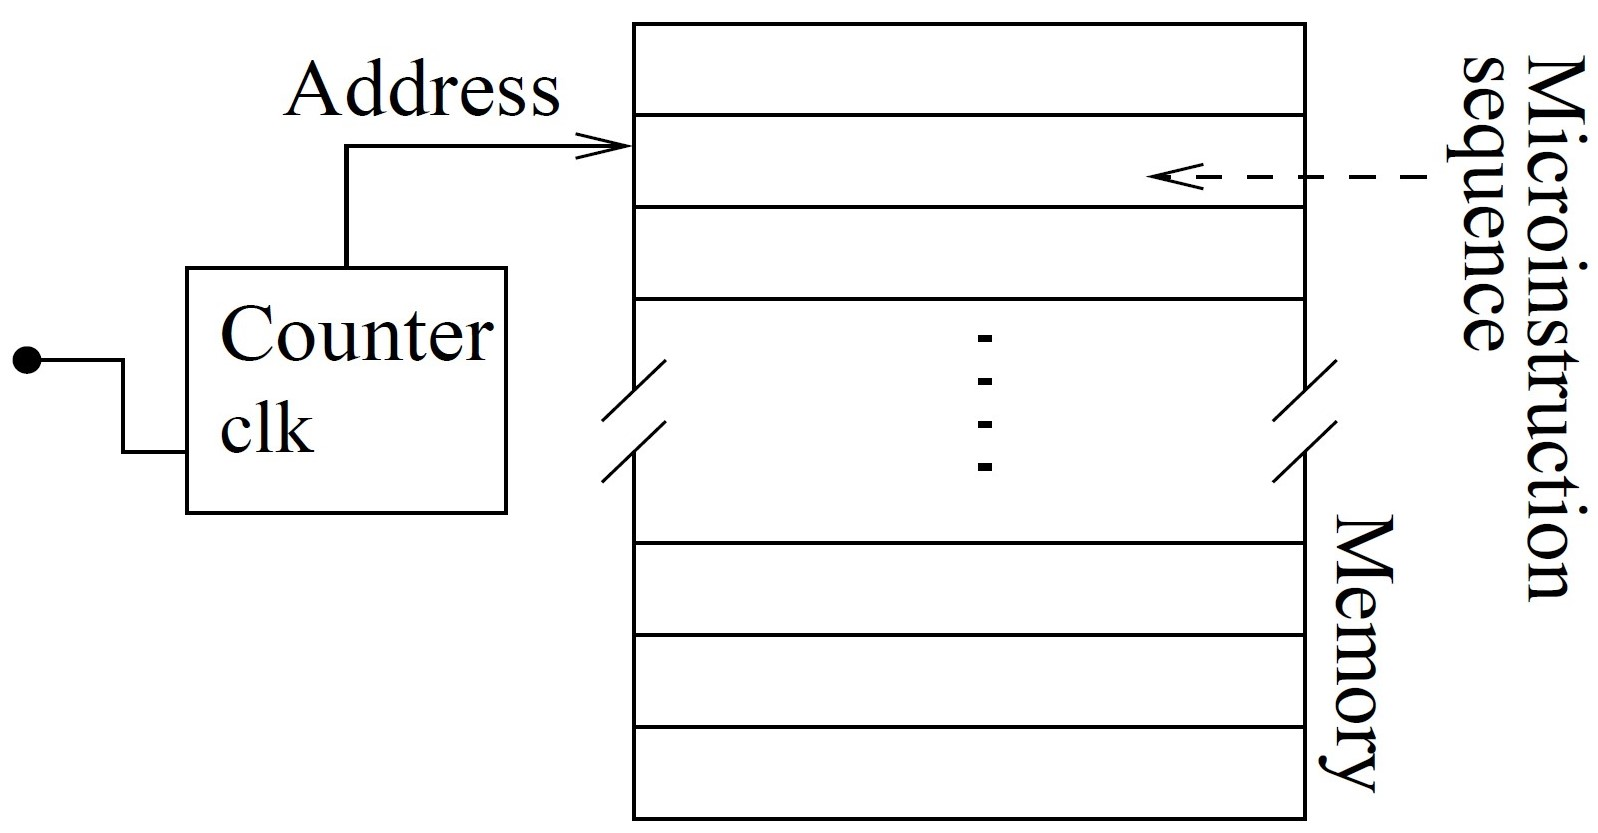
\includegraphics[width=\linewidth]{Pictures/Experiment 4/c-mem.jpg}
        \caption{Control Memory}
        \label{subFig:c-mem}
    \end{subfigure}
    \caption{Data Swap between A and B}
    \label{Fig:d-swap}
\end{figure}
\pagebreak

\subsection{Major Components/Modules Used}
\begin{enumerate}
    \item Registers
    \item Multiplexers and Decoders
    \item D Flip Flops
    \item Memory Module
\end{enumerate}

\subsection{Implementation}

\begin{figure}[h!]
    \centering
    \begin{subfigure}[b]{0.45\linewidth}
        \centering
        \frame{\includegraphics[width=\linewidth]{Pictures/Experiment 4/Imp-manual.jpg}}
        \caption{Data Swap}
    \end{subfigure}
    \begin{subfigure}[b]{0.45\linewidth}
        \centering
        \frame{\includegraphics[width=\linewidth]{Pictures/Experiment 4/Imp-cbus.jpg}}
        \caption{Common Bus}
    \end{subfigure}
    \begin{subfigure}[b]{\linewidth}
        \centering
        \frame{\includegraphics[width=0.9\linewidth]{Pictures/Experiment 4/Imp-cmem.jpg}}
        \caption{Control Memory}
    \end{subfigure}
    \caption{Implementation of Data Swap between A and B}
    \label{Fig:imp-d-swap}
\end{figure}

\subsection{Verification}   
\begin{enumerate}
    \item Successfully swapped content of A and B manually, using T as a temporary register.
    \item Successfully implemented common bus and implemented data swap on it.
    \item Successfully used Memory to automate the swapping procedure.
\end{enumerate}   

\subsection{Conclusion}
We hence realized register level data transfer using common bus and control memory.
\pagebreak

\section{Design of Sequence Counter for Processor Control Unit}
\subsection{Objective}
To build a mod-8 sequence counter for generation of control signals of a processor ALU.

\subsection{Theoretical Basis}
The instruction cycle of a CPU is shown in Figure \ref{fig:inst-cycle-CPU}. Assuming that each step is performed in an appropriately chosen clock period. A control unit for this CPU can be build around a modulo-8 sequence counter.

\begin{figure}[h!]
    \centering
    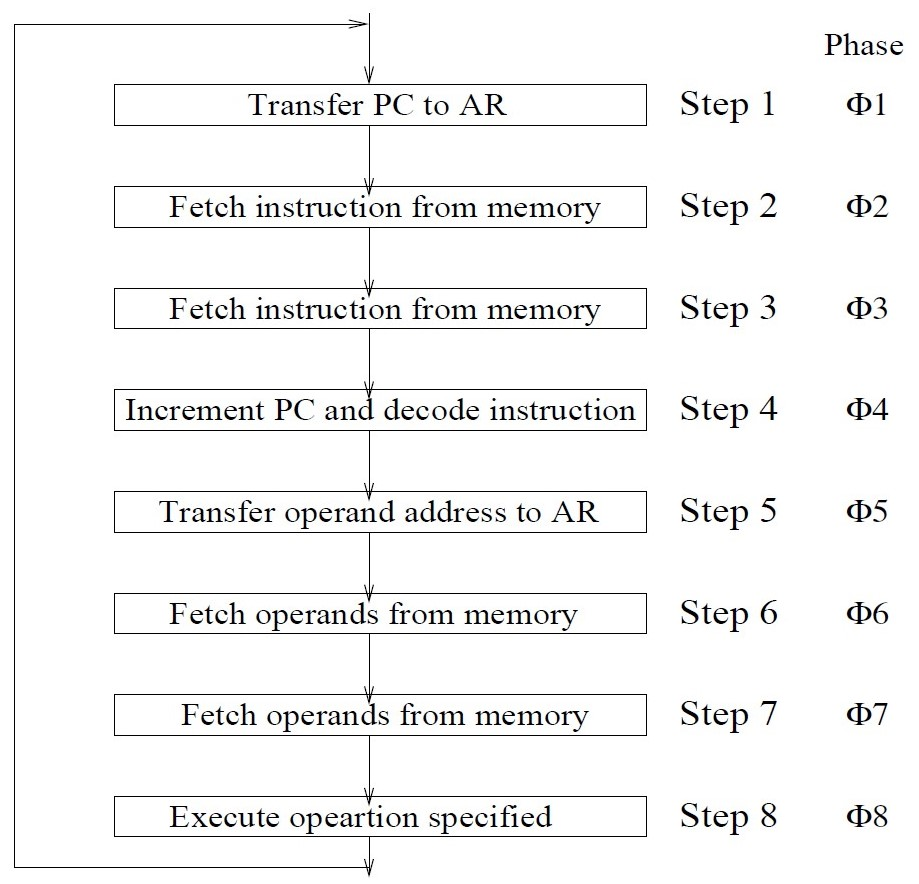
\includegraphics[width=0.5\linewidth]{Pictures/Experiment 5/inst-cycle.jpg}
    \caption{Instruction Cycle of CPU}
    \label{fig:inst-cycle-CPU}
\end{figure}

\noindent A modulo-8 counter counts input clock pulses from 000 to 111 and then sets to 000. The modulo-8 sequence counter can be designed with a modulo-8 counter and a 3-to-8 decoder. The decoder decodes the 3-bit binary code into a 1-bit binary code.

\subsection{Task and Design}
\begin{enumerate}
    \item Design Modulo-8 sequence counter as in figure \ref{Fig:des-mod8}.
    \item Design a combinational logic that takes the phase signals ($\phi_1$, $\phi_2$, $\phi_3$, $\phi_4$, $\phi_5$, $\phi_6$, $\phi_7$, $\phi_8$) as the input generates a sequence of signals to control the primitive operations of the ALU.
\end{enumerate}

\begin{figure}[h!]
    \centering
    \begin{subfigure}[b]{0.35\linewidth}
        \centering
        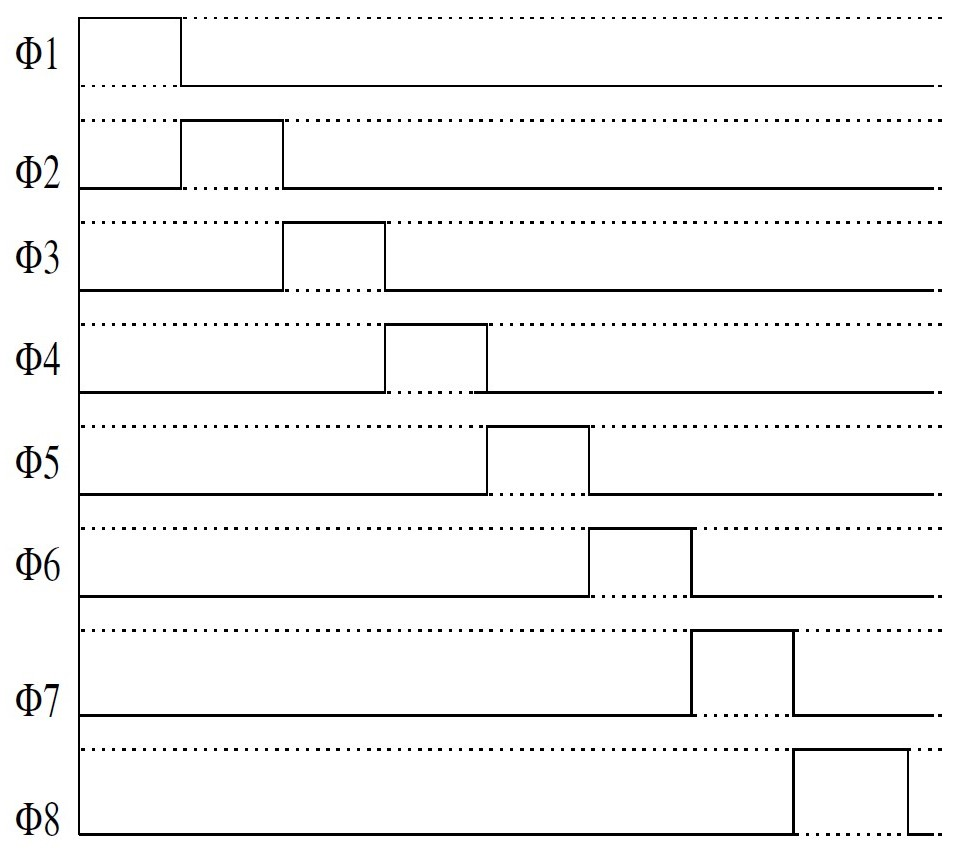
\includegraphics[width=\linewidth]{Pictures/Experiment 5/phase.jpg}
        \caption{Clock Pulses of $\phi_i$}
    \end{subfigure}
    \begin{subfigure}[b]{0.35\linewidth}
        \centering
        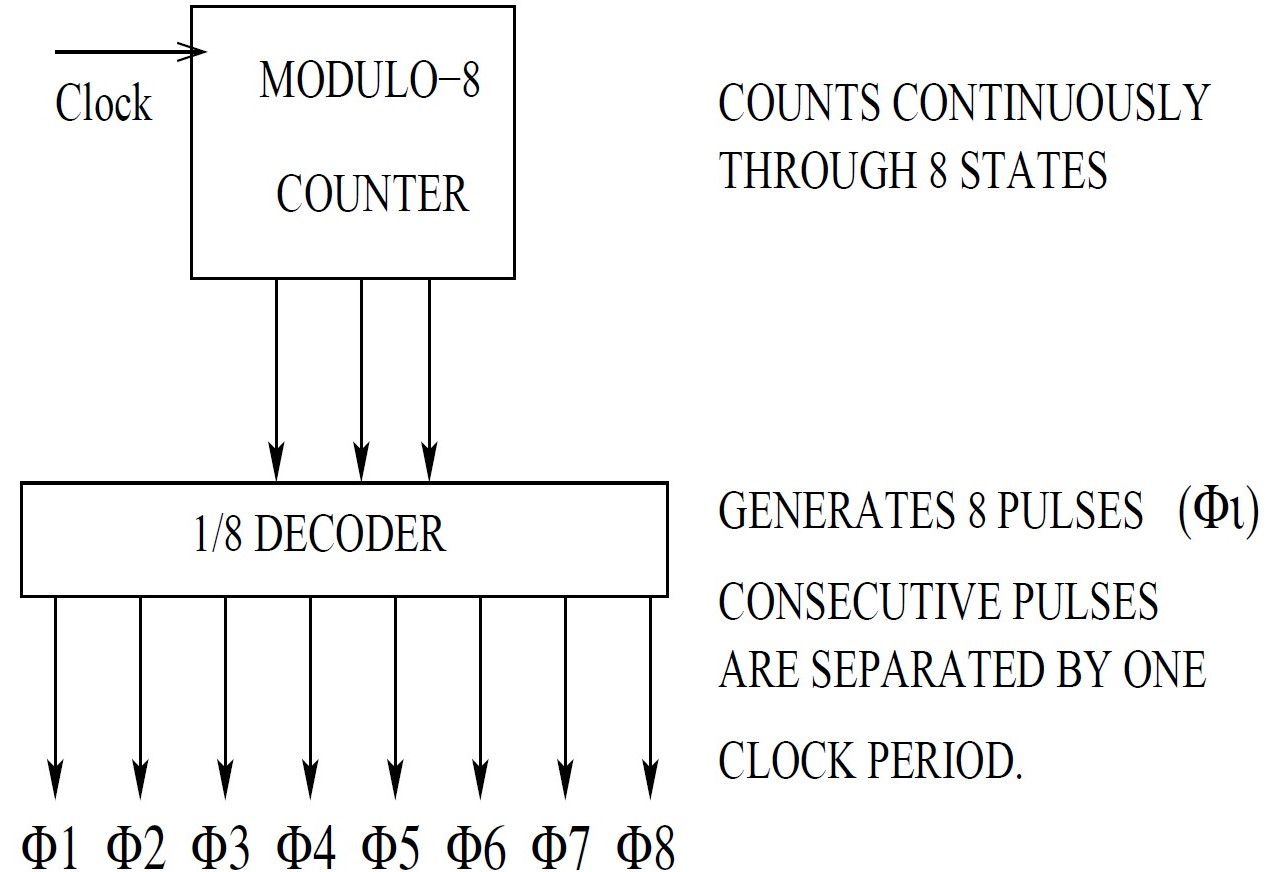
\includegraphics[width=\linewidth]{Pictures/Experiment 5/des-mod8-counter.jpg}
        \caption{Modulo-8 Sequence Counter}
    \end{subfigure}
    \caption{Design Of Modulo-8 Sequence Counter}
    \label{Fig:des-mod8}
\end{figure}
\pagebreak

\subsection{Major Components/Modules Used}
\begin{enumerate}
    \item A modulo-8 counter. The counter was constructed using 3 JK flip flops and 2 AND gate as there was no counter available in the simulator.
    \item One 3-to-8 decoder. The decoder was constructed using two 2-to-4 decoders as there was no 3-to-8 decoder available in the simulator.
    \item ALU Chip
\end{enumerate}

\subsection{Implementation}
\begin{figure}[h!]
    \centering
    \begin{subfigure}[b]{\linewidth}
        \centering
        \frame{\includegraphics[width=0.4\linewidth]{Pictures/Experiment 5/imp-mod8.jpg}}
        \caption{Implementation of Modulo-8 Sequence Counter}
    \end{subfigure}
    \begin{subfigure}[b]{\linewidth}
        \centering
        \frame{\includegraphics[width=0.4\linewidth]{Pictures/Experiment 5/imp-ALU.jpg}}
        \caption{ALU running from Modulo-8 Sequence Counter}
    \end{subfigure}
    \caption{Implementation of Sequence Counter to Drive ALU}
    \label{Fig:des-mod8}
\end{figure}

\subsection{Verification}
\begin{itemize}
    \item The modulo-8 counter designed in the simulator counts from 000 to 111 properly when simulated i.e. when the clock is turned on. It then sets it back to 000. The 3-to-8 decoder decodes the 3-bit binary code (000-111) and produces a single control signal at a time.
    \item The Control signal then properly drives the ALU 
\end{itemize}

\subsection{Conclusion}
A modulo-8 sequence counter with ALU is successfully designed and verified using the simulator.Hence, the given task is completed.
\end{document}